
\subsection{What we are protecting against}
What is the threat model?
Use some Set notation to make what is being protected more explicit.

What can we gaurantee with this threat model, and what sort of architecture
do we need to define to do this?

How can this be practically used in the real world?

\subsection{Tool-Flow}

What are the more concrete steps involved in getting this done?
What does the frontend look like (overview) and what about the backend,
is that mostly LegUp?

\begin{figure}[!t]
\centering
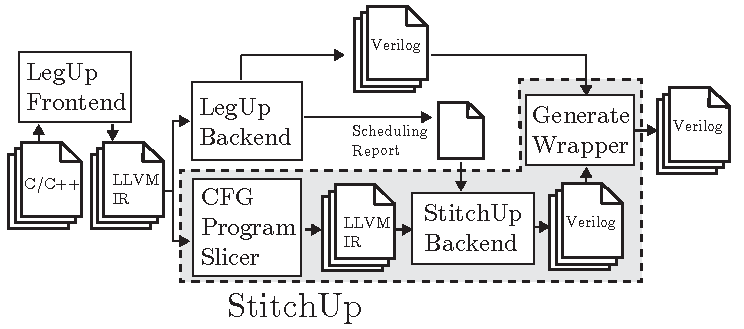
\includegraphics[width=2.5in]{./imgs/tool-flow.pdf}
\caption{Tool Flow Overview diagram}
\label{fig:tool_flow_diagram}
\end{figure}

This section will likely be quite small.
